%===========================================================
%                              Choix de thématique
%===========================================================
% Une des quatre options 'parallelisme', 'architecture', 'systeme' 
% 'tempsreel' doit être utilisée avec le style compas2021
\documentclass{article}

\usepackage{listings}
\usepackage{algorithmicx,fullpage}
\usepackage[noend]{algpseudocode}
\usepackage{algorithm,hhline}
\usepackage{graphicx}
\usepackage{wrapfig}
\usepackage{subcaption}
\usepackage{color}
\usepackage{float}
\definecolor{light-gray}{gray}{0.80}
%===========================================================
%                               Title
%===========================================================
\definecolor{dkgreen}{rgb}{0,0.6,0}
\definecolor{gray}{rgb}{0.5,0.5,0.5}
\definecolor{mauve}{rgb}{0.58,0,0.82}

\lstset{frame=tb,
  language=C,
  aboveskip=3mm,
  belowskip=3mm,
  showstringspaces=false,
  columns=flexible,
  basicstyle={\small\ttfamily},
  numbers=none,
  numberstyle=\tiny\color{gray},
  keywordstyle=\color{blue},
  commentstyle=\color{dkgreen},
  stringstyle=\color{mauve},
  breaklines=true,
  breakatwhitespace=true,
  tabsize=3
}
\lstset{emph={%  
    in%
    },emphstyle={\color{red}\bfseries}%
}%
\begin{document}
\bibliographystyle{plain}

\lstset{
  language=C,
  basicstyle=\tiny\ttfamily,
%  numbers=left,
%  xleftmargin=2em,
  frame=single,
%  framexleftmargin=2em,
  escapeinside={(*}{*)}
}

\title{Exploring vectorization and unrolling with SMT}

%\affiliation{\institution{Bordeaux Institute of Technology} \city{Bordeaux} \country{France}}
%\affiliation{\institution{Bordeaux Institute of Technology} \city{Bordeaux} \country{France}}
\author{Denis Barthou \and Edgar Baucher \and Ahmed-Manaf Dhamani \and William Jalby}
%\affiliation{\institution{University of Versailles Saint Quentin} \city{Versailles} \country{France}}


%\date{\today}

\maketitle



\section{Introduction}
High performance kernels require multiple optimizations, that can be performed by the compiler for many of them, and by the expert user for some of them. We do not
focus particularly on codes from libraries, but rather on kernels from
applications. One of the objectives is to study how to generate
efficient source code, while still keeping the code portable,
understandable by users and allowing composition. As a counterpart, we
may not wish to reach top performance but this would be suficient to
stay close to it (let us say 80\% of the top performance) if this
allows portability, maintenance and composability.

Many optimizations at the loop level and targeting cache/memory
hierarchy are well known and can be handled by dedicated compiler
optimizations. Let us focus here on code optimizations for codes that
run in a tile fitting in cache (or that does not have
reuse) and we assumed the code has been SIMDized by the user, resorting to a library such as the C++ MIPP
wrapper \cite{mipp} in order to ensure portability accross multiple architectures. We therefore focus on a very narrow optimization
space at compiler level, namely instruction
scheduling, loop transformations (within the tile) and
register allocation, all of them having been the subject of many related works in the past. For matrix product for instance, ATLAS \cite{atlas}, published 21 years ago, proposed automatic tuning of matrix product codes, including register blocking and loop transformations, but some initial work \cite{JalbyM86} tackles the matrix multiplication hand-tuning even 15 years before ATLAS. Since then, hardware mechanisms such as  out of order execution, register renaming have been expected to mitigate the effect of  instruction scheduling and register blocking  optimizations. This study has therefore the following objectives:
\begin{itemize}
\item Determine if there is any impact still of instruction scheduling at the source level on performance 
\item Determine if there is a simple criterion deciding the unrolling factor of a code, and if it is portable accross architectures, compilers
\end{itemize}


The
particularities of the source code kernels we consider are listed here:
\begin{itemize}
  \item Vector instructions will be parametrized by their length VL (expressed in elements) so the code should be generic and cover all possible Vector Lengths
\item All instructions will be not differentiated with respect to DP versus SP. 
\item All arithmetic instructions will operate between registers (à la ARM): no operand coming from memory can be used in an arithmetic instruction. The compiler still has the possibility to rewrite a load and a computation into a computation using an address. 
\item We will use a Vector Reduction (denoted VRED) instruction capable of summing all of the components of a vector register. Such an instruction is available in ARM ISA but currently it requires a chain of between 4 and 6 instructions on X86
\item The code to be duplicated (through unrolling) will be enclosed between curly brackets. 
\item The instruction selection for vectorized code is assumed to be done by the user through MIPP. Indeed, while efficient instruction selection methods exist in current compilers, this is still limited to linear algebra codes. MIPP (or existing alternatives) removes this issue by proposing a wider access to intrinsics SIMD instructions.
\end{itemize}

\section{Matrix product, stored row-wise}
The matrix code is a kernel for libraries, but still there may be occurences of special matrix sizes that are not perfectly addressed by libraries. We will start with small rectangular bloc sizes first, multiplying a matrix of size $BLOCKI\times BLOCKK$ by a matrix of size $BLOCKK \times BLOCKJ$. We provide to the compiler a very naive code, where the loop are ordered i,j,k, the vectorization is explicit through MIPP, and unrolling is achieved in the source code annotations. The objective is to compare the behavior of the different unrolling factors, and observe how it affects register blocking In the code presented in Fig.\ref{fig:gemm}

The unrolling on k
produces a sequence of FMAs. This does not improve ILP for FMA but
this enhances register reuse and can help to hide other instruction
latencies (loads).  There is no tail code on purpose, the sizes BI,
BJ, BK are adjusted to the unrolling factors, while still keeping the
global size of matrices A,B and C within 5\% of the chosen global
size, for all unrolling factors.  The unrolling factors from 1 to 15
have been explored to evaluate the capacity of the compilers to
allocate registers and reschedule. We have limited the exploration of
the register block size $UI*UJ+UI*UK+UJ*UK$ so that it does not exceed
twice the amount of SIMD registers (so 64 for AVX512, 32 for AVX), and
$UJ*VL$ should not exceed the size of the dimension BJ. Note that usually the number of physical registers exceed by more than a factor of two the number of virtual registers. The type of the elements are defined by \texttt{TYPE} . The above code
is written using a template mechanism that is instantiated
into C++ code for all unrolling factors.  The first machine of the
evaluation is an Intel Cascade Lake 6230R with AVX-512. The compilers
evaluated are, with flag -O3: icc version 19.1.3.304,  Clang 15 with 3 register allocation methods, greedy
(base), basic and PBQP, and GCC version 11.9. icc version 2021
(dpc++ OneAPI) is based on Clang 15 and does not exhibit any differences with Clang 15 greedy. 


\begin{figure}
  \begin{lstlisting}
for (int i=0;i<BLOCKI;i+=ui) {                
  for (int j=0;j<BLOCKJ;j+= uj*nv) {           
    { ii in [0,ui],jj in [0,uj]:
        mipp::Reg<TYPE> c_ii,jj;
        c_{ii,jj}.load(&C[(i + ii )*BLOCKJ + j + jj *nv]);
    }                
    for (int k=0;k<BLOCKK;k+= uk ) {            
      { ii in [0,ui],kk in [0,uk]:
          mipp::Reg<TYPE> a{{ ii }}{{ kk }};
          a_{ii,kk} = mipp::set1<TYPE>(A[(i + ii )*BLOCKK+k+ kk ]);
      }
      { jj in [0,uj],kk in [0,uk]:
          mipp::Reg<TYPE> b{{ kk }}{{ jj }};
          b_{kk,jj}.load(&B[(k+ kk )*BLOCKJ + j + jj*nv]);
      }    
      { ii in [0,ui], jj in [0,uj] :
          c_{ii,jj} = { k in [0,uk]: mipp::fmadd(a_ii,kk, b_kk,jj, } , c_ii,jj  { k in [0,uk]: ) };
      }
    }
    { ii in [0,ui],jj in [0,uj]:
        c_ii,jj.store(&C[(i+ ii )*BLOCKJ + j + ( jj )*nv]);      
    }
  }
}
  \end{lstlisting}
  \caption{Matrix product vectorized and unrolled\label{fig:gemm}. \texttt{in} constructs correspond to unrolled statements/expressions. }
\end{figure}


\subsection{Impact of unrolling factors}
For all plots in Fig.\ref{fig:cascadelake}, the same codes with the same vectorization expressed with MIPP are
compiled. All codes are tested 40 times, the best performance is shown. Only one memory allocation is used for all tests. Points shown in blue correspond to codes that should not require
more SIMD registers than the physical registers (32 for AVX-512, 16 for AVX2, shown by the vertical red line), whatever
the scheduling chosen by the compiler. This is not the case for codes
shown in red, some schedules may manage to use only registers while
others will require spill code. The graphs show performance w.r.t. the
cumulated register count and spill used by the code. For instance, a value of 40 registers and
spill used indicates that the compiler was able to use all 32
registers and 8 additional spaces on the stack for spill. With the exception of
GCC and icc 19.1.3, other compilers manage to allocate less than the number of registers for all
blue codes.

\begin{figure*}[h!]
%  \begin{subfigure}[h]{0.45\textwidth}
%  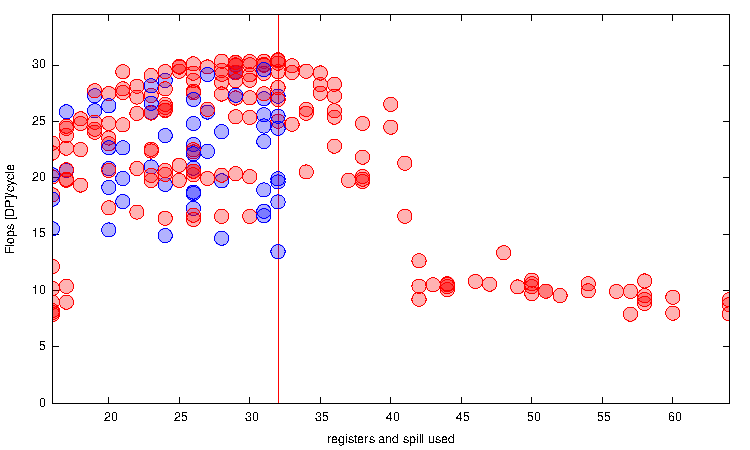
\includegraphics[width=\textwidth]{../benches/gemm/cascadelake-64x256x64/icc-2021.2.0.pdf}
%  \caption{icc 2021.2.0}
%  \end{subfigure}
  \begin{subfigure}[h!]{0.45\textwidth}  
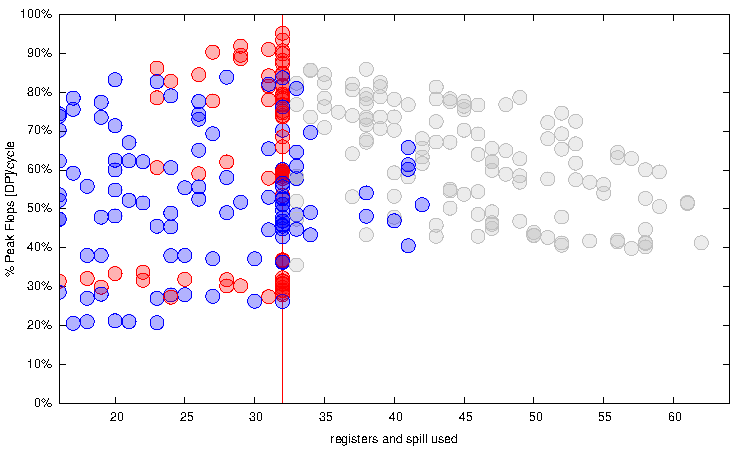
\includegraphics[width=\textwidth]{../benches/gemm/cascadelake-64x256x64/icc-19.1.3.pdf}
  \caption{Intel CascadeLake, AVX-512, icc 19.1.3}
  \end{subfigure}
  \begin{subfigure}[h!]{0.45\textwidth}  
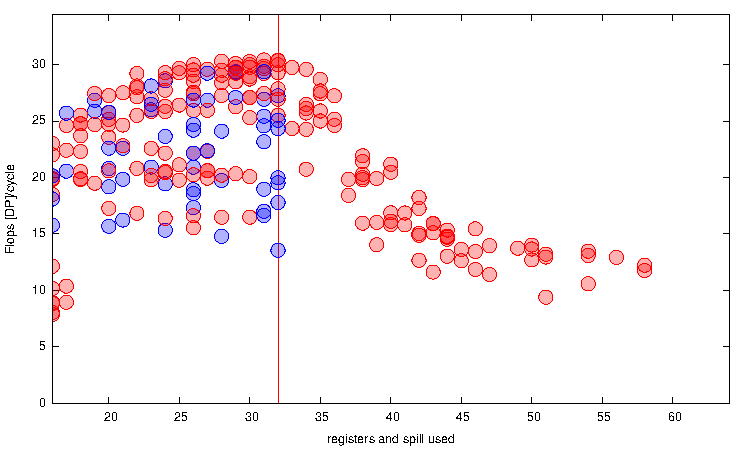
\includegraphics[width=\textwidth]{../benches/gemm/cascadelake-64x256x64/pbqp.pdf}
  \caption{Intel CascadeLake, AVX-512, Clang 15/PBQP}
  \end{subfigure}\\
  \begin{subfigure}[h!]{0.45\textwidth}  
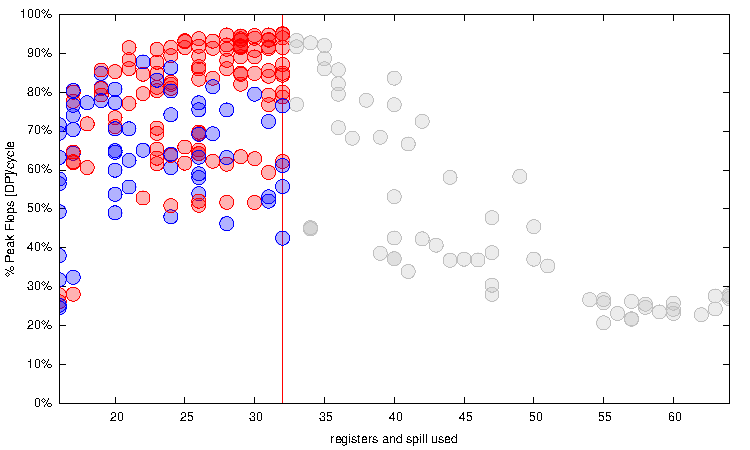
\includegraphics[width=\textwidth]{../benches/gemm/cascadelake-64x256x64/greedy.pdf}
  \caption{Intel CascadeLake, AVX-512, Clang 15/greedy}
  \end{subfigure}
  \begin{subfigure}[h!]{0.45\textwidth}  
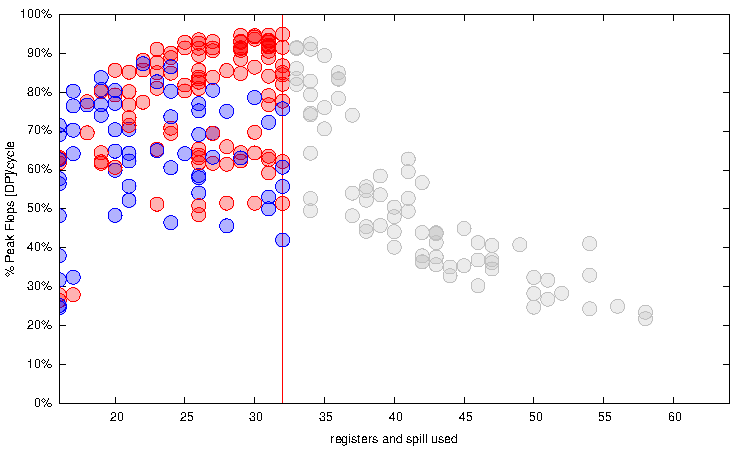
\includegraphics[width=\textwidth]{../benches/gemm/cascadelake-64x256x64/basic.pdf}
  \caption{Intel CascadeLake, AVX-512, Clang 15/basic}
  \end{subfigure}\\
  \begin{subfigure}[h!]{0.45\textwidth}  
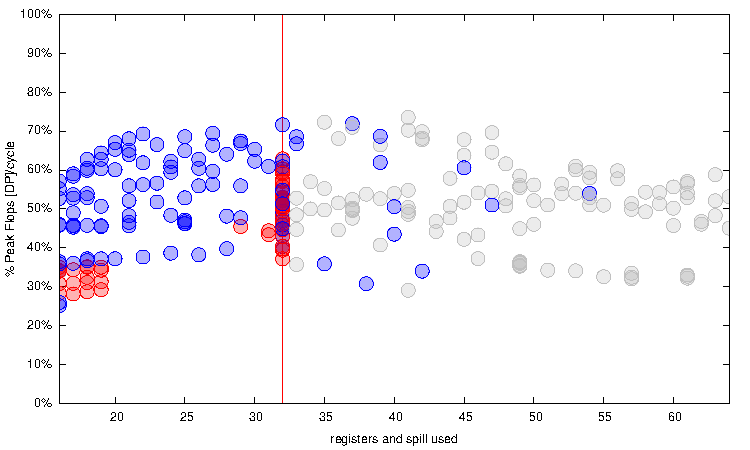
\includegraphics[width=\textwidth]{../benches/gemm/cascadelake-64x256x64/gcc-11.9.pdf}
  \caption{Intel CascadeLake, AVX-512, GCC 11.9}
  \end{subfigure}
  \caption{Block DGEMM Performance on AVX-512 architecture w.r.t. register and spill usage. Performance is given in \% of peak flops/cycle. The block (BI,BK,BJ) is 64x256x64. Each code represents a different register block size, obtained through the three unrolling factors. Codes with register block size lower than $32$ are in blue (should fit in registers whatever the schedule), other codes are in grey (with spill) and red (without spill).  \label{fig:cascadelake}}
\end{figure*}
\begin{figure*}[h!]
  \begin{subfigure}[h!]{0.45\textwidth}
  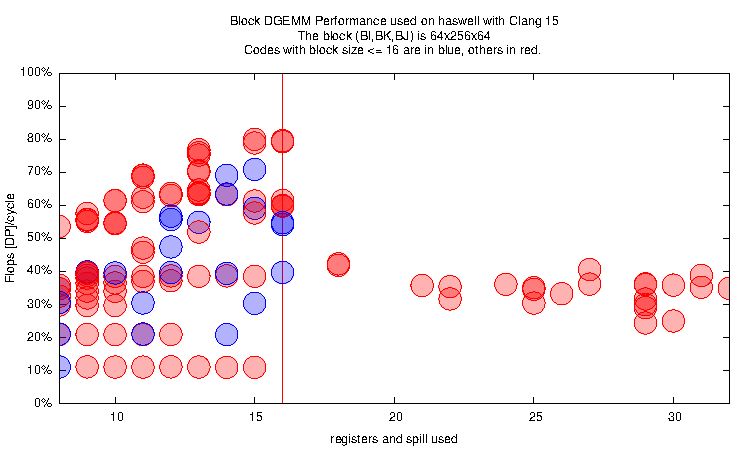
\includegraphics[width=\textwidth]{../benches/gemm/haswell-64x256x64/greedy.pdf}
  \caption{Intel Haswell, AVX2, Clang 15}
  \end{subfigure}
  \begin{subfigure}[h!]{0.45\textwidth}  
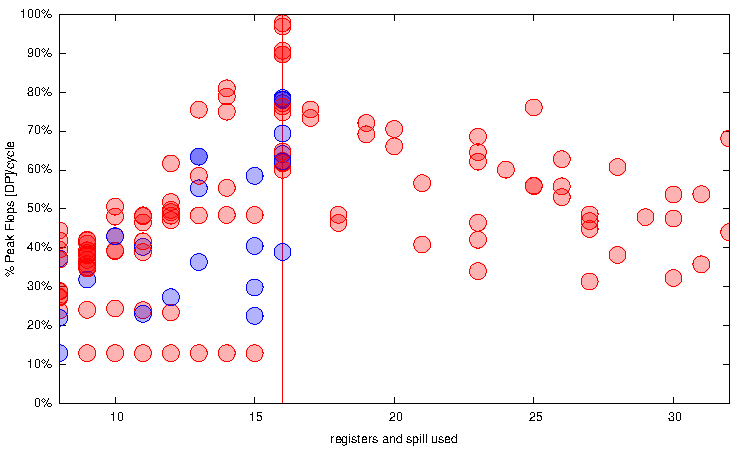
\includegraphics[width=\textwidth]{../benches/gemm/zen3-64x256x64/greedy.pdf}
  \caption{AMD Zen 3, AVX2, Clang 15$^*$}
  \end{subfigure}\\
  \begin{subfigure}[h!]{0.45\textwidth}  
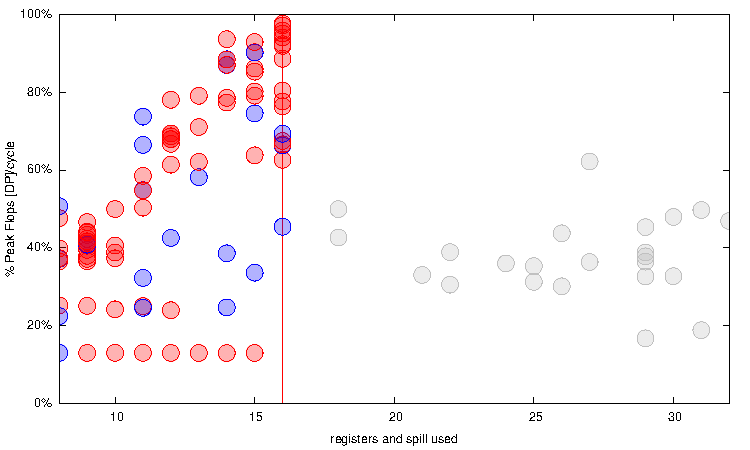
\includegraphics[width=\textwidth]{../benches/gemm/zen3-64x256x64/greedy-zen2.pdf}
  \caption{AMD Zen 2, AVX2, Clang 15$^*$}
  \end{subfigure}
  \caption{Block DGEMM Performance on AVX2 architectures w.r.t. register and spill usage. Performance is given in \% of peak flops/cycle. The block (BI,BK,BJ) is 64x256x64. Each code represents a different register block size, obtained through the three unrolling factors. Codes with register block size lower than $16$ are in blue (should fit in registers whatever the schedule), other codes are in grey (with spill) and red (without spill).  \label{fig:avx2}}
\end{figure*}
 

For AVX-512, different compilers are evaluated, and different register allocations for Clang. There is no significant difference between icc version 2021 and Clang
15, either greedy or PBQP register allocations. This is expected since
icc now is based on LLVM. GCC however fails significantly, reaching
only 24 flop/cycle while other compilers reach 30-31 flop/cycle.  For
the following experiments, only Clang 15 with greedy register
allocation is considered.

The best performing code is on AVX-512 and AVX2, with all compilers
with the exception of GCC, a code using exactly the maximum number of
registers, and correspond to a red dot: the block size exceeds the
size of vectors but there is no spill. This means the compiler creates
some artificial dependences by reusing SIMD registers among the
unrolled instructions. For GCC, the best performing code using 32
registers on AVX-512 is among the best performing codes, and it
corresponds to a blue dot. On all cases, \textbf{we observe that the range of
codes using all SIMD registers, no spill, covers a wide range of
performance, even if we focus on codes with red dots. Hence in order to
select the best performing codes, with running it, we need another
metric.}


\subsection{Correlation between compiler versions on Intel CascadeLake}

Figure \ref{fig:cascadelakecorrelation}  shows the correlation between the codes compiled by the three compilers on Intel CascadeLake AVX-512. One dot corresponds to the same source code, with the same unrolling factors. \textbf{The correlation between performance of a code accross different compilers is rather weak}, since the plot does not correspond to a diagonal. 

\begin{figure*}[h!]
  \begin{subfigure}[h]{0.45\textwidth}
  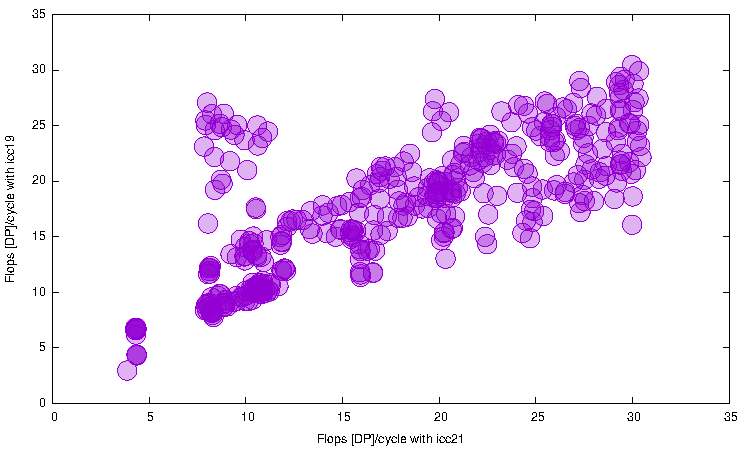
\includegraphics[width=\textwidth]{../benches/gemm/cascadelake-64x256x64/icc21xicc19.pdf}
  \caption{Clang 15 compared to icc 19.1.3}
  \end{subfigure}
  \begin{subfigure}[h]{0.45\textwidth}  
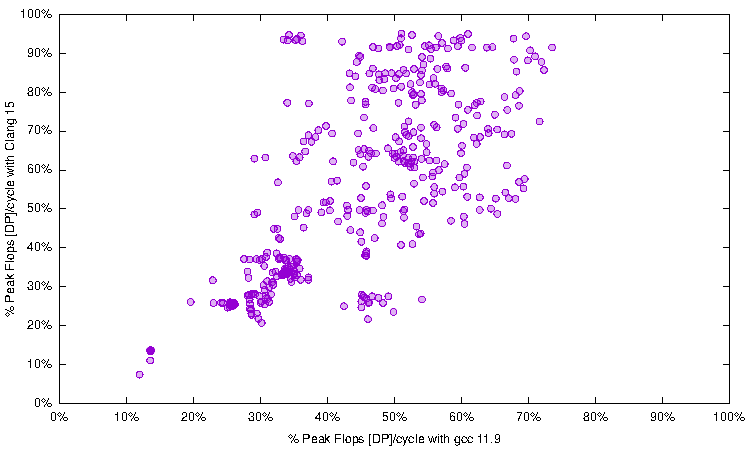
\includegraphics[width=\textwidth]{../benches/gemm/cascadelake-64x256x64/gccxgreedy.pdf}
  \caption{Clang 15 compared to gcc 11.9}
  \end{subfigure}

  \caption{(a) and (b) Correlation of code performance on CascadeLake between different compilers.\label{fig:cascadelakecorrelation}. In (a), the red dots correspond to codes that have a register block size of exactly 32. It implies that whatever the scheduling, it fits into registers.}
\end{figure*}
Tables in Figure \ref{fig:tables} provide additional insight by showing the
performance of the $14$  best performing  codes using exactly 32 registers, no spill, for each compiler. The
block size refers to the size taken by the input matrices manipulated
in the inner loop, in number of vectors. Sizes larger than 32 imply that the compiler has rescheduled loads during the computation and reuses SIMD registers. We observe that the best codes are different from one compiler to the other, there is no code outperforming the others.

In addition to the block sizes, the tables show also the expected parallelism degree (here obtained as the unrolling factors $ui*uj$). This metric is further explored in the following section.

\begin{figure*}[h!]
% For clang 15
{    \scriptsize
    \begin{tabular}{|c|c|c|c|}
      \hline
      \multicolumn{4}{|c|}{Code performance with Clang} \\
      \hline
      Unrolling & flop/cycle & block  & ILP\\
      ixkxj& in peak \% & size & \\
      \hline
14x1x2 & 93.59 & 44 & 28 \\
4x1x6 & 93.45 & 34 & 24 \\
5x3x4 & 93.34 & 47 & 20 \\
6x1x4 & 93.78 & 34 & 24 \\
6x2x3 & 93.84 & 36 & 18 \\
6x2x4 & 93.95 & 44 & 24 \\
5x1x5 & 94.79 & 35 & 25 \\
6x3x3 & 94.47 & 45 & 18 \\
6x3x4 & 94.53 & 54 & 24 \\
6x4x3 & 94.05 & 54 & 18 \\
7x2x3 & 94.81 & 41 & 21 \\
8x1x3 & 94.65 & 35 & 24 \\
7x3x3 & 95.05 & 51 & 21 \\
8x2x3 & 95.12 & 46 & 24 \\
\hline
\end{tabular}
% For icc
    \begin{tabular}{|c|c|c|c|}
      \hline
      \multicolumn{4}{|c|}{Code performance with icc 19.1.3} \\
      \hline
      Unrolling & flop/cycle & block  & ILP\\
      ixkxj& in peak \% & size & \\
      \hline
4x3x3 & 78.09 & 33 & 12 \\
3x2x6 & 79.18 & 36 & 18 \\
3x2x8 & 79.61 & 46 & 24 \\
3x1x8 & 81.90 & 35 & 24 \\
4x3x4 & 81.55 & 40 & 16 \\
7x2x2 & 83.77 & 32 & 14 \\
4x2x4 & 84.94 & 32 & 16 \\
6x2x3 & 84.73 & 36 & 18 \\
5x2x4 & 87.42 & 38 & 20 \\
4x2x5 & 88.23 & 38 & 20 \\
4x1x6 & 89.93 & 34 & 24 \\
10x1x2 & 90.70 & 32 & 20 \\
5x1x5 & 93.48 & 35 & 25 \\
6x1x4 & 95.23 & 34 & 24 \\
\hline
    \end{tabular}
% For gcc
    \begin{tabular}{|c|c|c|c|}
      \hline
      \multicolumn{4}{|c|}{Code performance with gcc 11.9} \\
      \hline
      Unrolling & flop/cycle & block  & ILP\\
      ixkxj& in peak \% & size & \\
      \hline
2x5x4 & 54.09 & 38 & 8 \\
3x6x2 & 54.83 & 36 & 6 \\
2x3x5 & 55.79 & 31 & 10 \\
2x2x6 & 57.52 & 28 & 12 \\
3x3x5 & 57.37 & 39 & 15 \\
3x5x4 & 57.08 & 47 & 12 \\
3x2x5 & 59.60 & 31 & 15 \\
3x5x3 & 59.15 & 39 & 9 \\
2x4x4 & 60.30 & 32 & 8 \\
3x4x4 & 60.33 & 40 & 12 \\
3x5x2 & 60.89 & 31 & 6 \\
3x3x4 & 62.91 & 33 & 12 \\
3x4x3 & 62.37 & 33 & 9 \\
5x3x2 & 71.70 & 31 & 10 \\
\hline
    \end{tabular}
}
\caption{Performance of the best 14 codes on Intel CascadeLake, AVX-512, with Clang15,  icc 19.1.3 and gcc 11.9. Only codes using 32 registers and 0 spill are considered here\label{fig:tables}. block size corresponds to $ui*uj+ui*uk+uk*uj$. $40$ means that the code requires $40$ zmm registers if all loads are scheduled before the computation. ILP corresponds here to $ui*uj$.}
\end{figure*}

\subsection{Impact of expected ILP}
The expected ILP, resulting from unrolling all three loops in a matrix multiply operation, is $ui * uj$. Indeed, the $uk$ unrolling factor only builds a longer sequence of FMA operations and is not expected to create additional ILP.
Figure \ref{fig:cascadelakeilp} shows the performance according to the parallelism expected from unrolling, on AVX-512 and AVX2 architectures. From this plot, we observe that for icc and Clang on AVX-512, the best codes result from a high ILP. On the contrary, for gcc on AVX-512, the code without spill with the highest expected ILP only reaches $42\%$ of the max performance (rightmost red dots). For AVX2 architectures, the rightmost red dots (no spill) do not correspond to the best performing code.
\textbf{The expected ILP does not seem to be a sufficient criteria to select the best performing code.}
\textbf{The reason  may be explained by the difference between the expected ILP, in theory, and the ILP actually obtained in the assembly code generated by the compiler.}
\begin{figure*}[h!]
%  \begin{subfigure}[h]{0.45\textwidth}
%  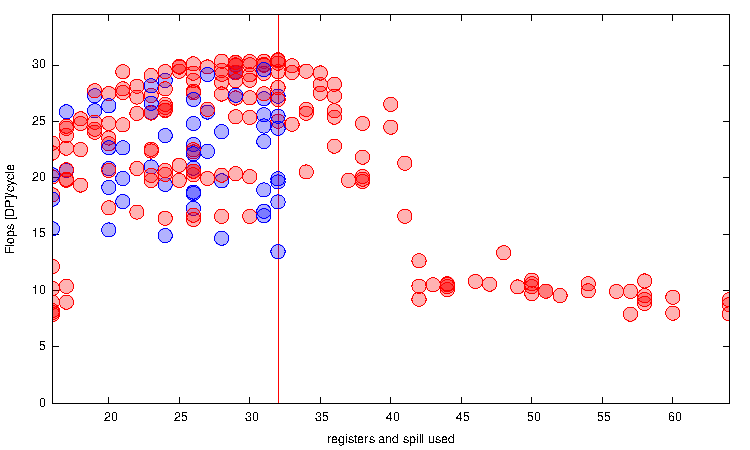
\includegraphics[width=\textwidth]{../benches/gemm/cascadelake-64x256x64/icc-2021.2.0.pdf}
%  \caption{icc 2021.2.0}
%  \end{subfigure}
  \begin{subfigure}{0.45\textwidth}  
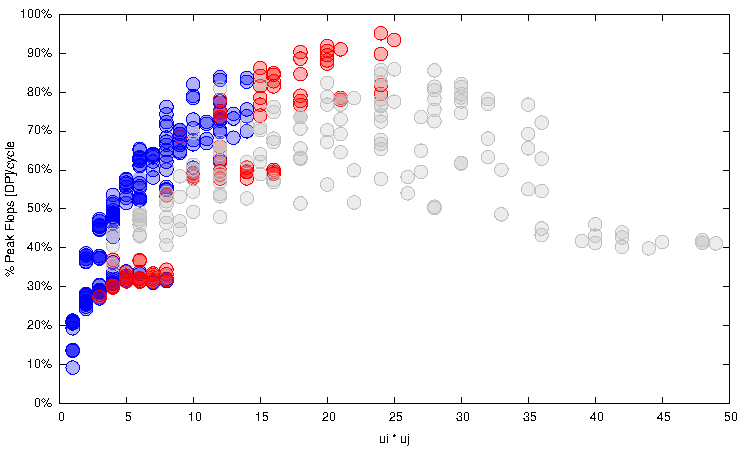
\includegraphics[width=\textwidth]{../benches/gemm/cascadelake-64x256x64/icc-19.1.3p.pdf}
  \caption{Intel CascadeLake, AVX-512, icc 19.1.3}
  \end{subfigure}
  \begin{subfigure}{0.45\textwidth}  
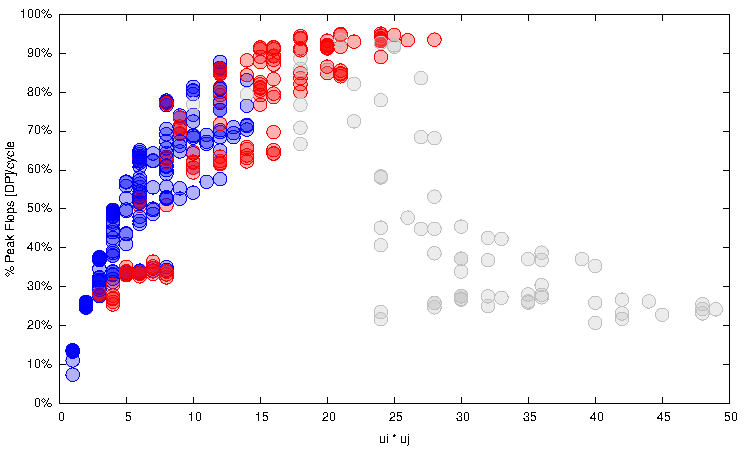
\includegraphics[width=\textwidth]{../benches/gemm/cascadelake-64x256x64/greedyp.pdf}
  \caption{Intel CascadeLake, AVX-512, Clang 15}
  \end{subfigure}\\
  \begin{subfigure}[h!]{0.45\textwidth}  
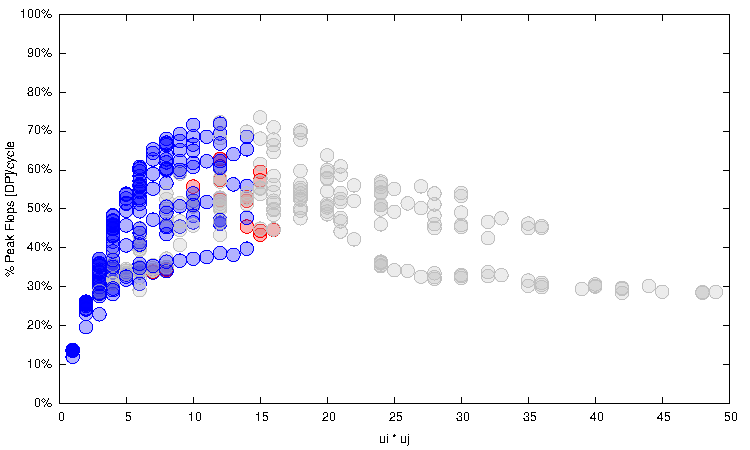
\includegraphics[width=\textwidth]{../benches/gemm/cascadelake-64x256x64/gcc-11.9p.pdf}
  \caption{Intel CascadeLake, AVX-512, GCC 11.9}
  \end{subfigure}
  \begin{subfigure}{0.45\textwidth}  
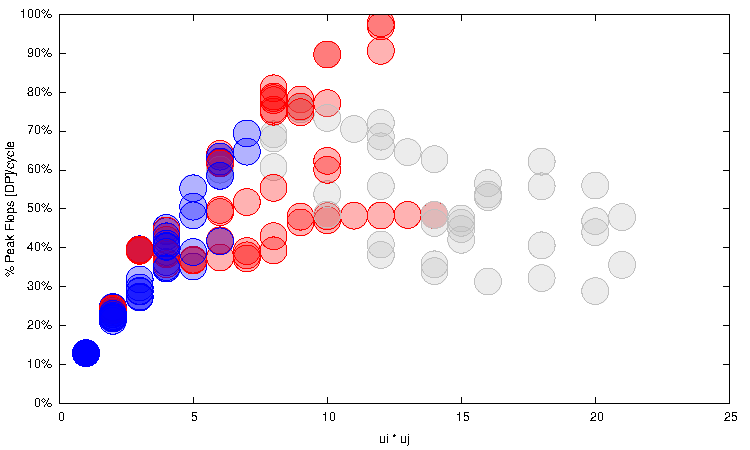
\includegraphics[width=\textwidth]{../benches/gemm/zen3-64x256x64/greedyp.pdf}
  \caption{AMD Zen 3, AVX2, Clang 15}
  \end{subfigure}\\
  \begin{subfigure}{0.45\textwidth}  
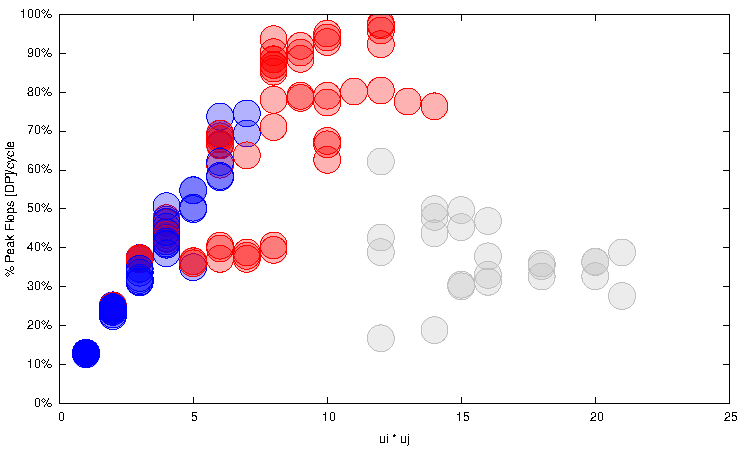
\includegraphics[width=\textwidth]{../benches/gemm/zen3-64x256x64/greedy-zen2p.pdf}
  \caption{AMD Zen 2, AVX2, Clang 15}
  \end{subfigure}
  \begin{subfigure}{0.45\textwidth}  
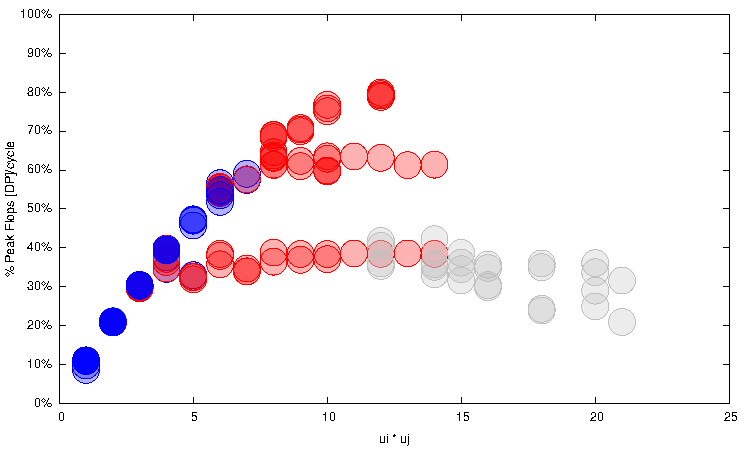
\includegraphics[width=\textwidth]{../benches/gemm/haswell-64x256x64/greedyp.pdf}
  \caption{Intel Haswell, AVX2, Clang 15}
  \end{subfigure}
  \caption{Block DGEMM Performance used on AVX-512 and AVX2 according to expected ILP. Performance is given in \% of peak flops/cycle. The expected ILP is the product of the unrolled factors $ui * uj$. The block (BI,BK,BJ) is 64x256x64. Each code represents a different register block size, obtained through the three unrolling factors. Codes with register block size lower than the number of registers are in blue (should fit in registers whatever the schedule), other codes are in grey (with spill) and red (without spill).\label{fig:cascadelakeilp}}
\end{figure*}

Finally, Figure \ref{fig:cascadelakeloc} shows for a given number of
source code lines, the performance obtained. Surprisingly, performance
culminates with 90 loc and then it degrades when the number of source
code lines. Note that the unrolling factor on k, creating a long
sequence of FMAs, is assumed to be on one single line of code.
\begin{figure*}[h!]
  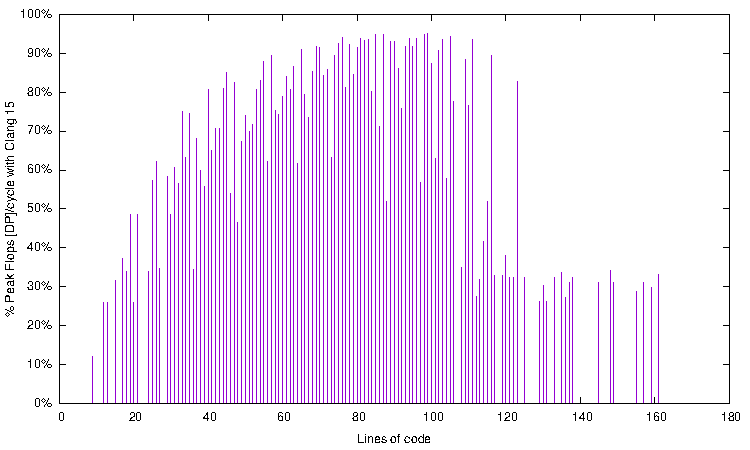
\includegraphics[width=0.45\textwidth]{../benches/gemm/cascadelake-64x256x64/icc21loc.pdf}
  \caption{Performance wrt lines of source code\label{fig:cascadelakeloc}}
\end{figure*}


\subsection{Impact of SMT on Cavium Arm ThunderX2 and Intel CascadeLake}
Simultaneous Multi-Threading (or hyperthreading) corresponds to the case where two threads (or more) are executed at the same time on the same core. The instructions are then intertwined, the functional units are put in common. SMT could be considered as a dynamic unrolling, especially interesting when facing codes calling library functions. The instructions of the functions are then intertwined, independently of the function scope.   

The codes considered are exactly the same as before (portability).  Due to the architecture of the processor, supporting an SMT of 4 for the Cavium, and SMT 2 for the Intel,  performance is compared for a single thread and performance with 4 and 2  threads resp., both on a single core. 

\begin{figure*}[h!]
  \begin{subfigure}[h]{0.45\textwidth}
  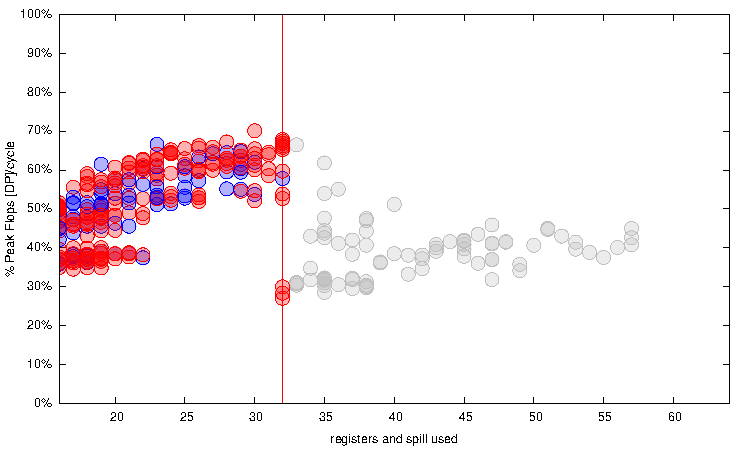
\includegraphics[width=\textwidth]{../benches/gemm/arm-64x256x64/greedy.pdf}
  \caption{Cavium Arm Thunder X2, NEON, Clang 15, no SMT}
  \end{subfigure}
  \begin{subfigure}[h]{0.45\textwidth}  
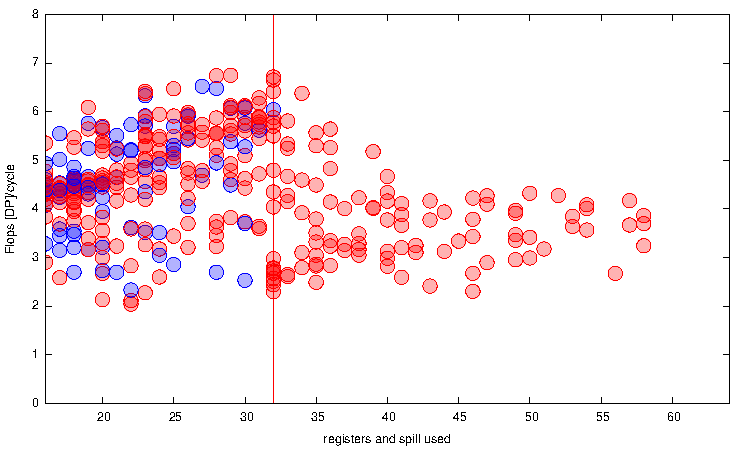
\includegraphics[width=\textwidth]{../benches/gemm/arm-64x256x64/openmp.pdf}
  \caption{Cavium Arm ThunderX2, NEON, Clang 15, SMT of 4}
  \end{subfigure}
    \caption{Block DGEMM Performance used on Cavium Arm ThunderX2 with (b) and without SMT (a). Performance is given in \% of peak flops/cycle (here 8). The block (BI,BK,BJ) is 64x128x64. Each code represents a different register block size, obtained through the three unrolling factors. Codes with register block size $\leq 32$ are in blue (fit in register whatever the schedule), others in red. \label{fig:arm}}
\end{figure*}
Performance 
The correlation between performance with and without SMT, both for Cavium Arm ThunderX2 (clang 15) and Intel CascadeLake (icc 19.1.3) are shown in Fig.\ref{fig:SMT}. For Arm, this is for 4 threads, for Intel this is for 2 threads. On Arm, SMT brings a $8\%$ improvement on the best code, and on Intel, the same percentage applies. However, the performance have been degraded when compiling with OpenMP flag (and running with 1 thread) compared to the non-OpenMP version.
\begin{figure*}[h!]
  \begin{subfigure}[h]{0.45\textwidth}  
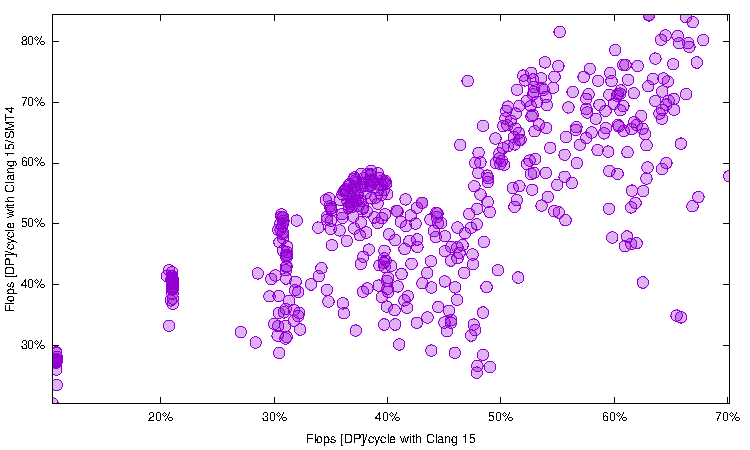
\includegraphics[width=\textwidth]{../benches/gemm/arm-64x256x64/clangxsmt.pdf}
  \caption{Correlation between Clang 15 without and with SMT4}
  \end{subfigure}
    \begin{subfigure}[h]{0.45\textwidth}  
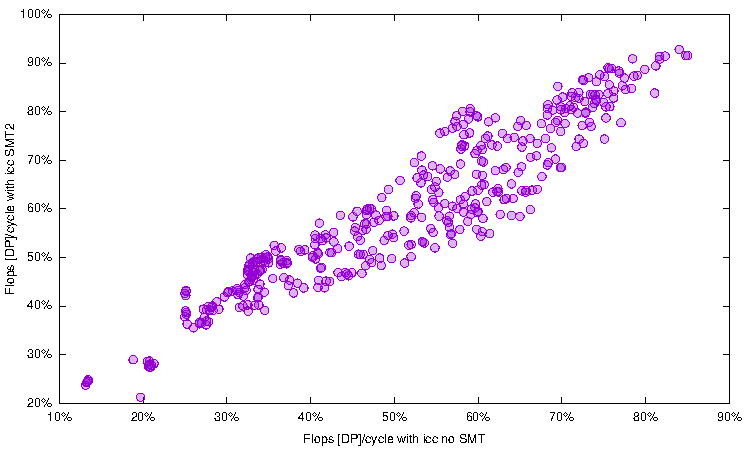
\includegraphics[width=\textwidth]{../benches/gemm/cascadelake-64x256x64/icc1thx2th.pdf}
  \caption{Correlation between icc without and with SMT2}
    \end{subfigure}
    \caption{Correlation between performance without SMT and with SMT, on Cavium Arm ThunderX2 (SMT4) and on Intel CascadeLake (SMT2). Performance is given in \% of peak flops/cycle. \label{fig:SMT}}
\end{figure*}

\textbf{For blocked  Gemm, it shows that SMT brings $8\%$ of performance, and the codes with good performance for SMT have good performance on 1 thread.} 
\section{Related Works}
\section{Conclusion}
\label{sec:conclusion}

\bibliography{biblio}

\end{document}
